%Correct the file name.
%X: book number
%Y: part number
%ZZZ: page number in three digits. So page 3 would be 003.

\documentclass[15pt]{amsbook}

\usepackage{../HBSuerDemir}	% ------------------------


\begin{document}

% ++++++++++++++++++++++++++++++++++++++
\hPage{b2p1/030}
% ++++++++++++++++++++++++++++++++++++++




% =======================================
\begin{enumerate}[label=\alph*]
    \item)  to have max error of $10^{ - 2}$ in sum s, how many terms should be taken?\\
\end{enumerate}

% =======================================

\underline{Solution.}
\begin{enumerate}[label=\alph*]
    \item)  Since $1\geq \frac{1}{2}\geq \frac{1}{3}...\geq \frac{1}{n}>... $ and $ \frac{1}{n}\rightarrow0,$ there is convergence.\\
    
    \item) $ \frac{1}{n+1} < \frac{1}{10^2} \Rightarrow n+1>100  \Rightarrow n>99 $ (100 terms)\\
\end{enumerate}

% =======================================

\section{\underline{SERRIES OF ARBITRARY TERMS}}

If a series is one of positive terms, one applies a test given for such series, if the series is alternating one applies LEBNIZ'test (test for alternating serries). For an arbitrary series the following theorem holds:

\underline{Theorem} A series

$$\sum_{i}^{} a_n = a_1+a_2+...+a_n+...$$
is convergent if the series
$$\sum_{i}^{} |a_n| = |a_1|+|a_2|+...+|a_n|+...$$
of absolute value is convergent.\\

\underline{Proof.} Let $s_n$,$S_n$ be the corresponding partial sums. The sum $s_n$ contains non negative and negative terms and we write\\

$s_n = P_n-Q_n$ , $S_n=P_n + Q_n$\\

where $P_n$ and $-Q_n$ are sums of positive and negative terms respectively.

$(P_n)$, $(Q_n)$ are monotone increasing sequences bounded above by $S = \lim_{} S_n $. Then $P_n \rightarrow P$, $Q_n \rightarrow Q$ and $S_n \rightarrow P + Q$. It follows that $s_n \rightarrow P - Q$
% =======================================






% =======================================================
\end{document}  

%==== templates ====

%==== environments ====

%\begin{figure}[htb]
%	\centering
%	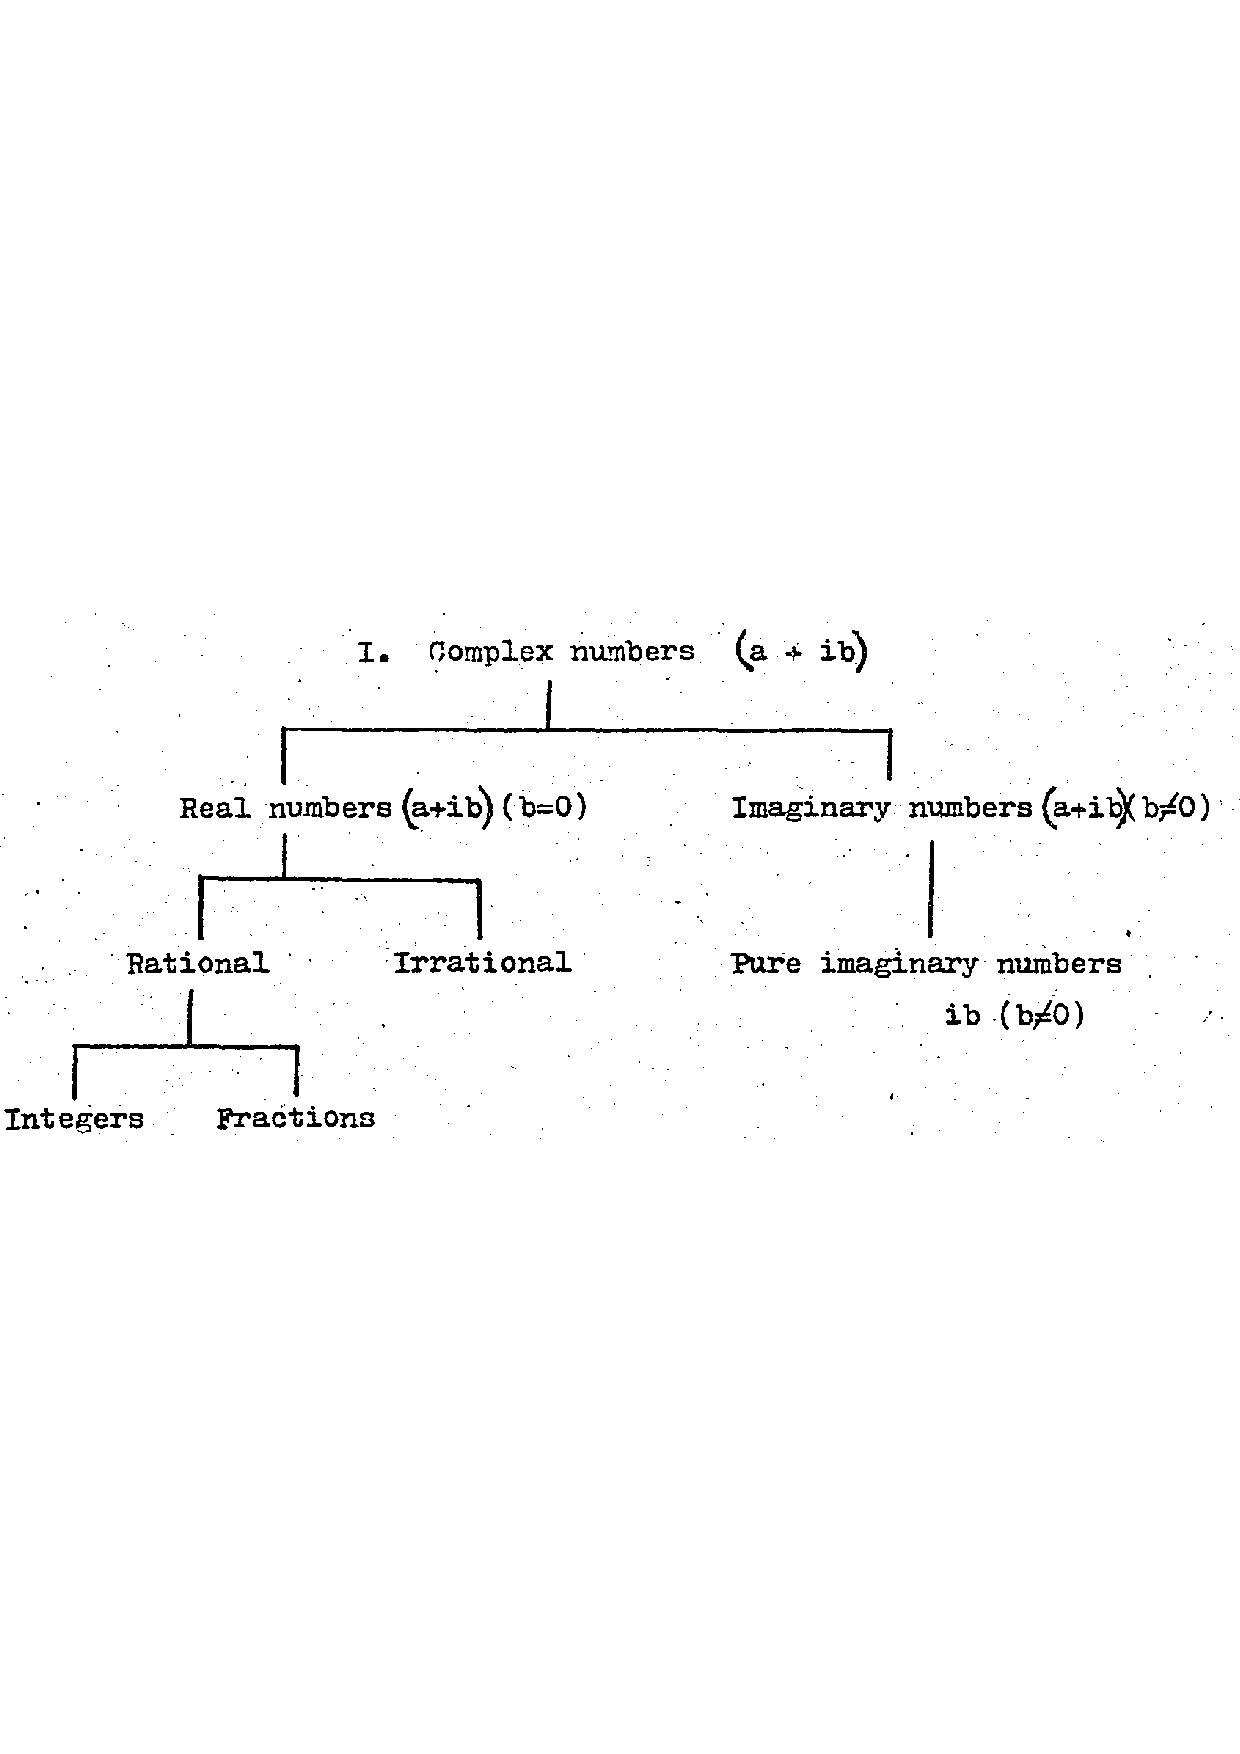
\includegraphics[width=0.9\textwidth]{images/SD-1-1p15A}
%	\caption{Classification of complex numbers}
%	\label{fig:classificationOfComplexNumbersA}
%\end{figure}

%\begin{center}
%\begin{tabular}{cc}
%\end{tabular}
%\end{center}

%\begin{exmp}
%\begin{hSolution}
%\end{hSolution}
%\end{exmp}

%\begin{hEnumerateAlpha}
%\end{hEnumerateAlpha}

%\begin{hEnumerateRoman}
%\end{hEnumerateRoman}

%$
%\begin{bmatrix}
%\end{bmatrix}
%$

%\frac{aaaa}{bbb}
%\frac{a_{n}}{b_{n}}
%\left( aaaa \right)
%\Longrightarrow

%\begin{multicols}{2}
%	bb
%\columnbreak
%	aa
%\end{multicols}
